\documentclass[11pt,a4paper]{article}
\usepackage[T1]{fontenc}
\usepackage[margin=2.3cm]{geometry}
\usepackage{amsmath,amssymb}
\usepackage{graphicx}
\usepackage[dvipsnames]{xcolor}
\usepackage{enumitem}
\usepackage[colorlinks=true,linkcolor=blue,urlcolor=blue]{hyperref}
\setlength{\parskip}{0.6em}
\setlength{\parindent}{0pt}
\begin{document}

\begin{center}{\LARGE\bfseries opengrid}\\[0.4em]{\large See how the grid balances supply and demand, and what power factor does.}\\[0.2em]\small PAN IIT OSS explainer \textbullet{} diploma / undergraduate to advanced undergraduate (levels 5-6)\end{center}

\section*{Why this exists}
An electricity grid is a balancing act: what is produced must equal what is used, second by second, and the frequency is the signal that tells us how well that balance is holding. This explainer follows the idea from a bar picture to AC power to a small frequency simulation.

\section*{The end goal}
See how the grid balances supply and demand, and what power factor does. The end goal is to see how the grid balances supply and demand and what power factor does, with simplified models you can run, test and extend. The models are for learning only and are never for operating a real grid.

\section*{How the three sessions build up}
\begin{enumerate}[nosep]
\item \textbf{Session 1: Supply must equal demand, every second} (Level 1, conceptual interactive model, 60 min).
\item \textbf{Session 2: AC power, power factor and why we use high voltage} (Level 2, mathematical engineering model, 75 min).
\item \textbf{Session 3: After a power station trips: frequency, inertia and droop} (Level 3, simulation and validation, 90 min).
\end{enumerate}

\section{Session 1: Supply must equal demand, every second}

\subsection*{A. Real-world problem}
When you switch on a kettle, a power station somewhere has to produce a little more electricity at that very moment. The grid has almost no storage, so what is produced must match what is used, second by second. What tells the whole country that demand has beaten supply? It is the frequency of the alternating current: 50 Hz when all is well, a little lower when demand wins. How big a shortage makes the frequency sag by 0.1 Hz?

\subsection*{B. Concept and theory}
The grid is one big spinning system. Every power station turbine and many motors turn in step at the grid frequency, 50 Hz in India and Europe. If generators supply less power than the load takes, the missing energy comes out of the rotating machines, they slow, and the frequency falls. If supply is higher than demand, they speed up and the frequency rises. Demand changes through the day (a morning bump, an evening peak and a night dip), so generators ramp up and down. Each unit has a size and a ramp rate (megawatts it can add per hour); cheap units are slow, flexible gas and hydro are fast. In Session 3 we derive the frequency dynamics; here we use their steady-state result for a small toy grid of 1000 MW: the frequency change is 50 Hz times the imbalance divided by (1000 MW times 21), where 21 is the grid stiffness 1/R + D of Session 3 (droop R = 0.05 gives 20, load damping D = 1 gives 1).

\begin{itemize}[nosep]
\item P\_supply: power produced by all generators (MW)
\item P\_demand: power taken by all loads (MW)
\item dP: imbalance, supply minus demand (MW)
\item f: grid frequency (Hz)
\item f0: nominal frequency, 50 (Hz)
\item BASE: size of the toy grid, 1000 (MW)
\item K: grid stiffness 1/R + D, equal to 21 (no unit)
\end{itemize}

\begin{equation*}
\Delta P = P_{\mathrm{supply}} - P_{\mathrm{demand}}
\end{equation*}

\begin{equation*}
f = f_0\left(1 + \frac{\Delta P}{\mathrm{BASE}\cdot K}\right),\qquad K = \frac{1}{R}+D = 21
\end{equation*}

\begin{equation*}
\text{a shortage of } 50\ \mathrm{MW}:\ \ \Delta f = -50\cdot\frac{50}{1000\cdot 21} = -0.119\ \mathrm{Hz}
\end{equation*}

\begin{center}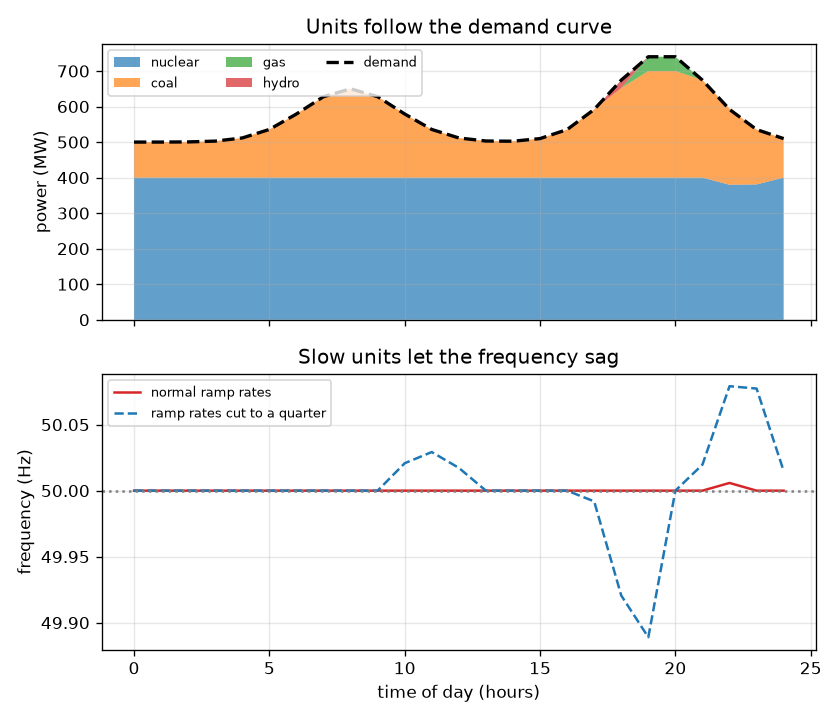
\includegraphics[width=0.85\linewidth]{figures/s01_day_dispatch.png}\\\small Generators following the daily demand curve; the lower panel shows how slow ramps let the frequency sag.\end{center}

\subsection*{E. Worked example}
Demand is 800 MW but the generators supply only 700 MW on the 1000 MW toy grid. What is the frequency?
\begin{enumerate}[nosep]
\item Imbalance = 700 - 800 = -100 MW (a shortage).
\item Frequency change = 50 * (-100) / (1000 * 21) = -0.238 Hz.
\item Frequency = 50 - 0.238 = 49.762 Hz.
\item Sanity check: half the shortage, 50 MW, should give half the fall: 0.119 Hz. It does.
\end{enumerate}
\textbf{Answer.} The frequency settles at 49.762 Hz, a drop of 0.238 Hz.

\subsection*{F. Questions}
\begin{enumerate}[nosep]
\item \textbf{Conceptual.} Why can the grid not simply store the extra power when demand is low, and why does a shortage show up as a lower frequency rather than a lower voltage?
\item \textbf{Numerical.} On the 1000 MW toy grid, demand is 600 MW and supply is 640 MW. What is the frequency?
\item \textbf{Graph and simulation interpretation.} In the frequency graph, what does the slope of the line mean, and what imbalance moves the frequency by 0.1 Hz?
\item \textbf{Design and optimisation challenge.} Design: the base units supply a fixed 600 MW and the flexible units can supply 0 to 600 MW. Demand through the evening is between 650 and 750 MW. Choose the flexible output for each demand so the frequency stays within 0.1 Hz of 50 Hz, and say what this tells you about how fast the flexible units must ramp.
\end{enumerate}

\section{Session 2: AC power, power factor and why we use high voltage}

\subsection*{A. Real-world problem}
A workshop takes 100 kW from a 400 V supply. With a power factor of 0.70 the cable and transformer must carry 357.1 A; with a power factor of 0.95 only 263.2 A for the very same useful power. Utilities charge extra for a low power factor, and long lines lose power as heat. What is power factor, how big a capacitor fixes it, and why do power lines use such high voltages?

\subsection*{B. Concept and theory}
With alternating current the current can lag the voltage by an angle phi, because motors and transformers store energy in magnetic fields. The useful power is P = V I cos(phi) (watts); the part that sloshes back and forth is the reactive power Q = V I sin(phi) (var); the wires must carry the apparent power S = V I (volt-amperes). They form a right triangle: S squared is P squared plus Q squared, and the power factor is cos(phi) = P / S. For the same real power, a lower power factor means a larger current: I = P / (V pf). A capacitor supplies reactive power locally, so the supply carries less. To lift the power factor from pf1 to pf2 at constant P the bank must supply Qc = P (tan phi1 - tan phi2); across a voltage V, a capacitor C supplies Qc = 2 pi f C V squared, so C = Qc / (2 pi f V squared). The same ideas apply to three-phase systems, where P = sqrt(3) V\_line I pf. Finally, a line of resistance R wastes I squared times R; for a fixed power, I = P / V, so loss = P squared R / V squared: ten times the voltage gives one hundredth of the loss.

\begin{itemize}[nosep]
\item V: RMS voltage (volt)
\item I: RMS current (ampere)
\item phi: angle by which current lags voltage (degrees)
\item P: real power (watt (W) or kW)
\item Q: reactive power (var or kvar)
\item S: apparent power (VA or kVA)
\item pf: power factor, cos(phi) (no unit)
\item Qc: reactive power from the capacitor (var or kvar)
\item C: capacitance (farad (microfarad))
\item R: line resistance (ohm)
\end{itemize}

\begin{equation*}
P = VI\cos\varphi,\qquad Q = VI\sin\varphi,\qquad S = VI,\qquad S^2 = P^2+Q^2,\qquad \mathrm{pf}=\cos\varphi=\frac{P}{S}
\end{equation*}

\begin{equation*}
I = \frac{P}{V\,\mathrm{pf}}
\end{equation*}

\begin{equation*}
Q_c = P\,(\tan\varphi_1-\tan\varphi_2),\qquad C=\frac{Q_c}{2\pi f V^2}
\end{equation*}

\begin{equation*}
P_{\mathrm{loss}} = I^2R = \frac{P^2R}{V^2\,\mathrm{pf}^2}
\end{equation*}

\begin{center}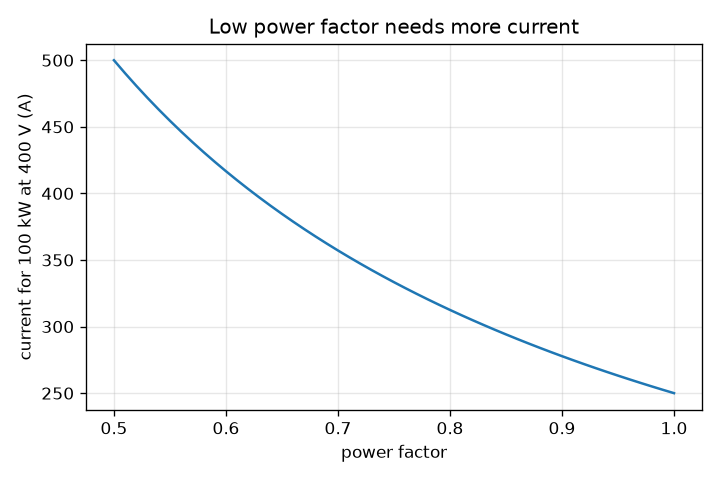
\includegraphics[width=0.85\linewidth]{figures/s02_current_vs_pf.png}\\\small Current for 100 kW at 400 V against the power factor.\end{center}

\subsection*{E. Worked example}
A 100 kW single-phase load on 400 V has pf 0.70. Find its current, the capacitor needed to reach pf 0.95, the capacitance at 50 Hz, and the new current.
\begin{enumerate}[nosep]
\item Current before: I = 100000 / (400 * 0.70) = 357.1 A.
\item tan(phi1) = tan(acos 0.70) = 1.0202 and tan(phi2) = tan(acos 0.95) = 0.3287.
\item Qc = 100 kW * (1.0202 - 0.3287) = 69.15 kvar.
\item C = 69150 / (2 pi * 50 * 400\textasciicircum{}2) = 0.001376 F = 1376 microfarad.
\item Apparent power after: S = 100 / 0.95 = 105.3 kVA, so I = 105260 / 400 = 263.2 A (down from 357.1 A).
\end{enumerate}
\textbf{Answer.} Qc = 69.15 kvar, C = 1376 microfarad, and the current falls from 357.1 A to 263.2 A.

\subsection*{F. Questions}
\begin{enumerate}[nosep]
\item \textbf{Conceptual.} Why does a low power factor waste capacity even though the reactive power does no useful work, and how does a capacitor help?
\item \textbf{Numerical.} A 30 kW single-phase load on 230 V has pf 0.8. Find its current, its reactive power, and the current if the pf were corrected to 1.
\item \textbf{Graph and simulation interpretation.} From the current-against-pf graph (100 kW, 400 V), what are the currents at pf 1 and pf 0.5, and what does that tell you?
\item \textbf{Design and optimisation challenge.} Design: a 50 kW load has pf 0.75 and must reach 0.95 at 400 V, 50 Hz. Find the exact capacitor size and capacitance. A supplier only stocks a 30 kvar bank: what pf does it give? Discuss the trade-offs.
\end{enumerate}

\section{Session 3: After a power station trips: frequency, inertia and droop}

\subsection*{A. Real-world problem}
A large power station suddenly trips and the grid loses 5 percent of its generation. Demand has not changed, so the rotating machines start to slow. How fast does the frequency fall, how low does it go, and where does it settle? And why do grid operators worry as more solar and wind (which have no big spinning mass) replace conventional plants? This is a toy illustration of the real study done by system operators.

\subsection*{B. Concept and theory}
Treat the whole grid as one aggregate generator with stored kinetic energy. The inertia constant H is the stored energy in seconds of rated power (about 5 s is typical for a conventional grid). Let dw = (f - f0) / f0 be the per-unit frequency deviation and dP the sudden loss (per unit). The swing equation is 2H d(dw)/dt = Pm - dP - D dw, where D is the damping from loads that use less power at lower frequency. Primary governor control with droop R (about 5 percent typical) raises the mechanical power as the frequency falls: Pm follows -dw / R, here with a combined turbine and governor lag Tg of 5 s. A fast battery can add power in proportion to the deviation, up to its size B, with a short lag. Two hand formulas test the solver: right after the loss the governor has not moved, so the rate of change of frequency is RoCoF = -f0 dP / (2H); once everything settles, the derivative is zero and Pm = -dw / R, giving df = -f0 dP / (1/R + D). Less inertia (more solar and wind) means a faster and deeper fall. A three-bus DC power flow (a stretch topic) solves the linear system B theta = P for the bus angles, and each line carries (theta\_i - theta\_j) / x.

\begin{itemize}[nosep]
\item H: inertia constant (s)
\item dw: per-unit frequency deviation (f - f0) / f0 (no unit)
\item dP: sudden generation loss, per unit on the generation base (pu)
\item D: load damping, 1 (pu)
\item R: governor droop, 0.05 (pu)
\item Pm: extra mechanical power from the governor (pu)
\item Tg: governor and turbine lag, 5 (s)
\item B: battery size (pu)
\item x: line reactance (pu)
\item theta: bus voltage angle (radian)
\end{itemize}

\begin{equation*}
2H\,\frac{d(\Delta\omega)}{dt} = P_m + P_b - \Delta P - D\,\Delta\omega,\qquad \Delta\omega=\frac{f-f_0}{f_0}
\end{equation*}

\begin{equation*}
T_g\,\frac{dP_m}{dt} = -\frac{\Delta\omega}{R} - P_m
\end{equation*}

\begin{equation*}
\mathrm{RoCoF} = -\frac{f_0\,\Delta P}{2H},\qquad \Delta f_{\infty} = -\frac{f_0\,\Delta P}{1/R + D}
\end{equation*}

\begin{equation*}
B\,\boldsymbol{\theta} = \mathbf{P},\qquad P_{ij} = \frac{\theta_i-\theta_j}{x_{ij}}
\end{equation*}

\begin{center}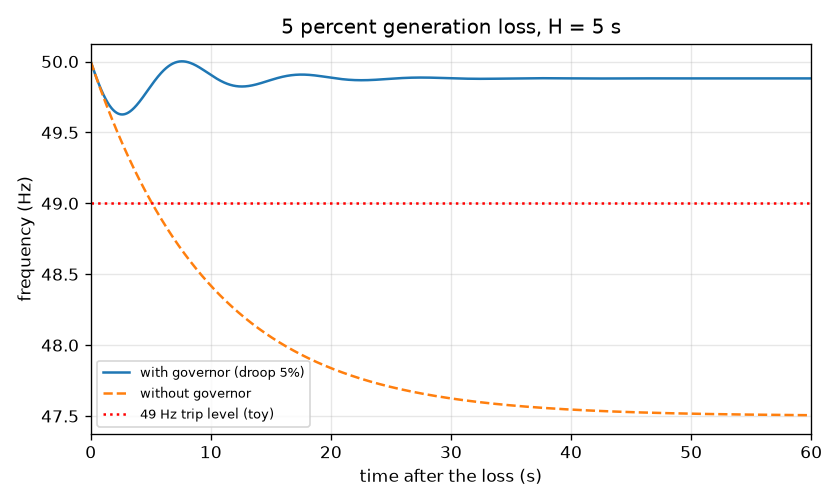
\includegraphics[width=0.85\linewidth]{figures/s03_frequency_response.png}\\\small A 5 percent loss at H = 5 s: with governor (nadir 49.627 Hz, settles at 49.881 Hz) and without (47.500 Hz).\end{center}

\subsection*{E. Worked example}
A 5 percent loss hits a grid with H = 5 s, D = 1 and droop R = 0.05. Find the initial RoCoF and the settled frequency by hand, then compare with the RK4 simulation.
\begin{enumerate}[nosep]
\item Initial RoCoF = -f0 dP / (2H) = -50 * 0.05 / (2 * 5) = -0.250 Hz/s.
\item Stiffness 1/R + D = 20 + 1 = 21.
\item Final deviation = -50 * 0.05 / 21 = -0.119 Hz, so the settled frequency is 49.881 Hz.
\item Without a governor the final deviation is -50 * 0.05 / 1 = -2.5 Hz, so 47.500 Hz.
\item The RK4 simulation gives a start slope of about -0.249 Hz/s, a settled value of 49.881 Hz with the governor and 47.500 Hz without; the nadir with the governor is 49.627 Hz.
\end{enumerate}
\textbf{Answer.} RoCoF is -0.250 Hz/s, the frequency settles at 49.881 Hz with the governor (47.500 Hz without it), and the lowest point is 49.627 Hz.

\subsection*{F. Questions}
\begin{enumerate}[nosep]
\item \textbf{Conceptual.} Why does a grid with a lot of solar and wind (little spinning mass) see a faster and deeper frequency fall after the same loss?
\item \textbf{Numerical.} An 8 percent loss hits a grid with H = 4 s. Find the initial RoCoF. Then for a 5 percent loss with droop R = 0.04 and D = 1, find the settled frequency.
\item \textbf{Graph and simulation interpretation.} In the inertia figure (10 percent loss), compare the initial slopes for H = 2 s and H = 5 s, and say which curve crosses 49 Hz.
\item \textbf{Design and optimisation challenge.} Design: after an 8 percent loss on a grid with H = 3 s the nadir must stay at or above 49.5 Hz. The nadir with no battery is 49.266 Hz. Find the smallest fast battery (in steps of 0.005 pu), and discuss what else could achieve it.
\end{enumerate}

\section{Real-world mini-project}
\textbf{How much fast battery keeps the frequency above 49.5 Hz?.} A low-inertia grid (H = 3 s) must survive the sudden loss of 8 percent of its generation without the frequency falling below 49.5 Hz. The governors alone are not enough. Use \texttt{simulate\_frequency} and \texttt{smallest\_battery} from Session 3 to find the smallest fast battery, in steps of 0.005 per unit. This is a toy study for learning, not a grid design.

\section{The path ahead}
\begin{enumerate}[nosep]
\item \textbf{Session 4: Synthetic inertia from a battery.} A battery model with power proportional to RoCoF and a power limit, added to the swing equation.
\item \textbf{Session 5: Limited governor headroom.} The governor output clipped to a reserve limit, with a settled-value formula.
\item \textbf{Session 6: Under-frequency load shedding.} Staged shedding steps at set frequencies added to the simulation.
\item \textbf{Session 7: AC power flow with voltage and reactive power.} A three-bus AC power flow solved iteratively.
\item \textbf{Session 8: Estimate inertia from a noisy trace.} A fitting routine that recovers H from a noisy simulated event.
\end{enumerate}

\section{Answers and hints}

\subsection*{Session 1}
\begin{enumerate}[nosep]
\item \textbf{Conceptual.} Hint: Think about where the energy comes from in the first seconds, and what is spinning. Solution: Large-scale storage is expensive and the grid is built to deliver power as it is made, so supply must follow demand. When supply is short, the missing energy is taken from the kinetic energy of the spinning generators and motors, so they slow down; the frequency is their common speed. Voltage is controlled separately (by reactive power, Session 2). A surplus does the opposite and the frequency rises.
\item \textbf{Numerical.} Hint: Use f = 50 * (1 + dP / (1000 * 21)) with dP = supply - demand. Solution: dP = +40 MW (a surplus). Frequency = 50 * (1 + 40 / 21000) = 50 + 0.095 = 50.095 Hz. It is above 50 Hz, as expected for a surplus.
\item \textbf{Graph and simulation interpretation.} Hint: The slope is the change in frequency per MW of imbalance. Solution: The slope is 50 / 21000 = 0.002381 Hz per MW. A change of 0.1 Hz needs 0.1 / 0.002381 = 42 MW of imbalance. The line falls to the right because more demand means more shortage.
\item \textbf{Design and optimisation challenge.} Hint: You need supply within about 42 MW of demand at every moment. Solution: Flexible output should be demand minus 600, within 42 MW: about 50 MW at 650 MW demand and about 150 MW at 750 MW demand. So the flexible units must be able to add about 100 MW over the hours between, and follow it closely; if they ramp too slowly the gap exceeds 42 MW and the frequency leaves the 0.1 Hz band. Trade-off: fast units (gas, hydro, batteries) are more expensive than slow base units.
\end{enumerate}

\subsection*{Session 2}
\begin{enumerate}[nosep]
\item \textbf{Conceptual.} Hint: Think about what the wires and transformers must carry. Solution: Wires and transformers carry the current, and the current follows the apparent power S, not just the real power P. Reactive power adds to the current without adding useful work, so for the same P the current is larger (I = P / (V pf)), which heats the wires more (I squared R) and uses up capacity. A capacitor supplies the reactive power next to the load, so the supply does not have to carry it.
\item \textbf{Numerical.} Hint: I = P / (V pf). Q = P tan(acos pf). Solution: I = 30000 / (230 * 0.8) = 163.0 A. Q = 30 * tan(36.87 degrees) = 22.5 kvar. At pf 1: I = 30000 / 230 = 130.4 A. Sanity check: the current is lower and the ratio is 0.8.
\item \textbf{Graph and simulation interpretation.} Hint: Evaluate I = P / (V pf). Solution: At pf 1 the current is 250 A and at pf 0.5 it is 500 A, twice as big. The curve rises steeply at low pf, so the saving from correcting from 0.5 to 0.7 is much larger than from 0.9 to 1.
\item \textbf{Design and optimisation challenge.} Hint: Qc = P (tan phi1 - tan phi2). With 30 kvar installed, the remaining reactive power is Q1 - 30 kvar. Solution: Exact: Qc = 27.66 kvar, which is 550 microfarad. The load has Q1 = 44.10 kvar; with 30 kvar installed, 14.10 kvar remains and pf = 50 / sqrt(50\textasciicircum{}2 + 14.10\textasciicircum{}2) = 0.9624, a little better than 0.95 but it over-corrects slightly at light load (leading current is bad). Trade-offs: bigger banks cost more, over-correction risks voltage rise and resonance, so engineers use stepped banks that switch with the load.
\end{enumerate}

\subsection*{Session 3}
\begin{enumerate}[nosep]
\item \textbf{Conceptual.} Hint: Look at where H enters the RoCoF formula. Solution: Less spinning mass means a smaller H. The initial rate of change is -f0 dP / (2H), so a smaller H gives a steeper fall; the governors need several seconds to react, so a faster fall also reaches a deeper low point before they catch up. The settled value does not depend on H, only on droop and damping.
\item \textbf{Numerical.} Hint: RoCoF = -f0 dP / (2H). Final = f0 - f0 dP / (1/R + D). Solution: RoCoF = -50 * 0.08 / (2 * 4) = -0.5 Hz/s. For the second part, 1/R + D = 25 + 1 = 26 and the deviation is -50 * 0.05 / 26 = -0.096 Hz, so the frequency settles at 49.904 Hz.
\item \textbf{Graph and simulation interpretation.} Hint: Use the RoCoF formula for each curve. Solution: H = 2 s: -50 * 0.10 / 4 = -1.25 Hz/s. H = 5 s: -50 * 0.10 / 10 = -0.5 Hz/s. The H = 2 s curve is 2.5 times steeper and dips to 48.921 Hz, below the 49 Hz trip level; the H = 5 s curve bottoms out at 49.253 Hz and does not cross.
\item \textbf{Design and optimisation challenge.} Hint: Run smallest\_battery(0.08, 3.0) and print the nadir for the sizes just below it. Solution: The smallest battery is 0.035 pu, which gives a nadir of 49.531 Hz; 0.030 pu falls short. Alternatives: more inertia (synchronous condensers), a smaller largest loss, stiffer (lower) droop, or a faster governor. Trade-offs: a battery responds in a fraction of a second but costs money per MW and has limited energy; extra inertia is slower to add but helps the first second.
\end{enumerate}

\section{How to join}
Read \texttt{CONTRIBUTING.md} in the repository, then pick an issue labelled \texttt{good first issue}. Repository: \url{https://github.com/KrunalPanchal1995/opengrid}

\end{document}
